%%%%%%%%%%%%%%%%%%%%%%%%%%%%%%%%%%%%%%%%%%%%%%%%%%%%%%%%%%%%%%%%%%%%%%%%%%%%%%%%%%%%

\section{Recursão}

\subsection{Recursão}
\begin{frame}[fragile]

\frametitle{Recursão}

\begin{itemize}

    \item A \textit{recursão} é um importante conceito da matemática e presente em muitas  linguagens
    de programação. Exemplo: LISP, Haskell, etc

    \pause
    \item Permite expressar conceitos complexos em uma sintaxe abstrata, mas  simples de ler.
    \pause
    \item Uma regra é dita recursiva quando ela faz auto-referência.
    
    \pause
    \item Em Picat, a recursão pode ser usada sob uma notação em \textit{lógica} ou \textit{funcional}
    
    \pause
    \item A funcional apresenta muita clareza ao código!
\end{itemize}

%\pause
%\centering
%
\includegraphics[scale=0.5]{figures/Recursao.png}
  
\end{frame}

%%%%%%%%%%%%%%%%%%%%%%%%%%%%%%%%%%%%%%%%%%%%%%%%%%%%%%%%%%%%%%%%%%%%%%%%

\begin{frame}[fragile]

\frametitle{Conceitos de Recursividade via Exemplos -- I}

\begin{block}{Somatório dos $N$ naturais}

 O somatório dos \emph{n}  primeiros  números naturais é recursivamente 
 definido como a soma de todos \emph{n-1} números, mais o termo \emph{n}. 
 Ou seja:

    \[
    S(n)=\left \{
    \begin{tabular}
        [c]{ll}
        $1$ & para $n=1$ \\
        $S(n-1) + n $ & para $n \geqslant 2$ e $n \in \mathbb{N}$
    \end{tabular}
    \right.
    \]
    
    Ou seja:
    
    \[
    S(n)=
    \begin{tabular}[c]{cc}
        $\underbrace{1+2+3+.....+(n-1)}$ &  $  + n$\\
        $S(n-1)$ &
    \end{tabular}
    \]
\end{block}            

\end{frame}

\begin{frame}[fragile]
\frametitle{Conceitos de Recursividade via Exemplos -- II}


\begin{block}{Fatorial}

O Fatorial de um número $n$ é definido  recursivamente pela
 multiplicação do fatorial do termo $n-1$ por $n$. 
  O fatorial só pode ser calculado para números positivos. 
  Adicionalmente, o fatorial de $0$ é igual a 
  $1$ por definição.
    \[ 
    Fat(n)=\left\{
    \begin{tabular}[c]{ll}%
        $1$ & para $n = 0$\\
        $Fat(n-1) . n$ & para $n\geqslant1$ e $n \in \mathbb{N}$
    \end{tabular}
    \right.
    \]
    
    Portanto:
    
    \[
    Fat(n)=
    \begin{tabular}
        [c]{cc}%
        $\underbrace{1\ast2\ast3 . ..... . (n-1)}$ & $ .  \ n$\\
        $Fat(n-1)$ &
    \end{tabular}
    \]

\end{block}    
\end{frame}


\begin{frame}[fragile]
\frametitle{Conceitos de Recursividade via Exemplos -- III}

\begin{block}{Sequência Fibonacci}

A sequência Fibonacci é uma sequência de números calculada a partir da soma dos
dois últimos números anteriores desta. Ou seja o $n-esimo$ termo da Sequência Fibonacci é definido como a soma dos termos $n-1$ e $n-2$. Como fato ou definição: os dois primeiros termos, $n = 0$ e $n = 1$, são respectivamente, $0$ e $1$.
      
      \[
      Fib(n)=\left\{
      \begin{tabular}[c]{ll}%
          $0$ & para $n = 0$\\
          $1$ & para $n = 1$\\
          $Fib(n-1) + Fib(n-2)$ & para $n\geqslant1$ e $n \in \mathbb{N}$
      \end{tabular}
      \right.
      \]
 
\end{block}    
\end{frame}

%%%%%%%%%%%%%%%%%%%%%%%%%%%%%%%%%%%%%%%%%%%%
\begin{frame}[fragile]

\frametitle{Conceitos de Recursividade via Exemplos -- IV}

  \begin{itemize}
      
      \item Podemos perceber algo em comum entre estas três regras, todas tem uma ou mais
      condições que sempre tem o mesmo valor de retorno, ou seja, todas tem uma \textit{regra de  aterramento}.
      
      \pause
      \item Uma condição de \textit{aterramento} é uma condição onde a chamada recursiva da regra
      acaba (pára ou termina).
      
       \pause
      \item Caso uma regra não tenha uma \textit{regra de aterramento}, poderá ocorrer uma recursão infinita deste regra, ou seja, são feitas infinitas chamadas recursivas
      da regra.
  \end{itemize}

\end{frame}

%%%%%%%%%%%%%%%%%%%%%%%%%%%%%%%%%%%%%%%%%%%%
\begin{frame}[fragile]

\frametitle{Exemplos}

Numa visão funcional, estas regras matemáticas podem ser transcritas em Picat como:

    \begin{lstlisting}[frame=single]
fatorial(0) = 1.
fatorial(1) = 1.
fatorial(n) = n * fatorial(n-1).
    \end{lstlisting}

    \begin{lstlisting}[frame=single]
fibonacci(0) = 0.
fibonacci(1) = 1.
fibonacci(n) = fibonacci(n-1) + fibonacci(n-2).
    \end{lstlisting}

    \begin{lstlisting}[frame=single]
somatorio(0) = 0.
somatorio(1) = 1.
somatorio(n) = n + somatorio(n-1).
    \end{lstlisting}

\end{frame}

%%%%%%%%%%%%%%%%%%%%%%%%%%%%%%%%%%%%%%%%%%%%%%%%%%%%%%%%%%%%%%%%%%%%%%%%%%%%%%

\begin{frame}[fragile]

\frametitle{Recursão Infinita}

    \begin{itemize}
        \item Caso a definição do fatorial fosse modificada para:
        
        \[
        Fat(n)= 
        \begin{tabular}[c]{ll}
            $Fat(n-1)\ast n$, &$\forall n \in \mathbb{N}$ ou $\forall n \geq 0$
        \end{tabular}
        \]
        \pause
        \item Teríamos um caso de \textit{recursão infinita}, pois a regra Fatorial continuaria
        a ser chamada com $n < 0$
        
        \item Nesse caso haveria um erro, pois estaria tentando executar algo indefinido.
        
    \end{itemize}

\end{frame}

%%%%%%%%%%%%%%%%%%%%%%%%%%%%%%%%%%%%%%%%%%%%%%%%%%%%%%%%%%%%%%%%%%%%%%%%%%%%%%


\begin{frame}[fragile]

\frametitle{Exercício}

Para os exemplos anteriores, reescreva-os
as formulações sob uma visão
\textit{lógica} e  \textit{procedural}.

\end{frame}


%%%%%%%%%%%%%%%%%%%%%%%%%%%%%%%%%%%%%%%%%%%%%%%%%%%%%%%%%%%%%%%%%%%%%%%%%%%%%%%%%%%%%%%%%%

\subsection{\textit{Backtracking}}
\begin{frame}[fragile]

\frametitle{\textit{Backtracking}}
\begin{itemize}
  \item O mecanismo de \textit{backtracking} é bem conhecido por algumas linguagens de programação

 % \pause 
 % \item Backtracking é um tipo de algoritmo que representa um refinamento da busca por força bruta,
%   em que múltiplas soluções podem ser eliminadas sem serem explicitamente examinadas.
  
  \pause 
  \item Em Picat, o \textit{backtracking} é controlável e é habilitado pelo símbolo
  \verb!?=>! no escopo da regra. 

\end{itemize}

\end{frame}

\begin{frame}[fragile]
\frametitle{Ilustrando o \textit{Backtracking} -- 01}

\begin{figure}[!htb]
\begin{center}
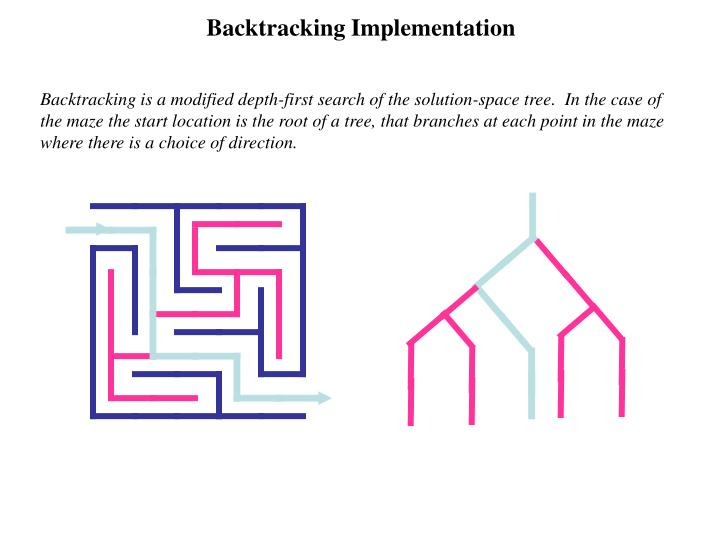
\includegraphics[width=0.80\textwidth, height=0.90\textheight]{figures/ilustra_backtracking_01.jpg}
%\caption{Realizar buscas com regiões reduzidas -- promissoras (regiões factíveis de soluções)}
\end{center}
\end{figure}
\end{frame}


\begin{frame}[allowframebreaks=0.7]
\frametitle{\textit{Backtracking}}

Basicamente o procedimento do \textit{Backtracking} é definido por:

\begin{enumerate}

\item Inicia-se por  um casamento de um predicado \textit{backtrackable} $p$ com um outro predicado $p$.

\item Segue-se a execução da regra $p$, executando a instância das variáveis da \underline{esquerda para direita}.
 \textbf{Exemplo} (ilustrativo):\\
      \texttt{p(X1,X2,X3, ....., Xn) ?=> q1(X1), q2(X2), ...., qn(Xn).} 

\item Caso ocorra uma falha durante a execução da regra $p$,
 o compilador busca re-instanciar as variáveis do corpo de $p$ que falharem. Esta tentativa segue uma ordem:\\ 
  $q1(X1) \rightarrow q2(X2)\rightarrow ....\rightarrow qn(Xn)$, até a variável $Xn$
%, incluindo aquelas indexadas a partir de um domínio.
%, com a única exceção sendo variáveis instanciadas a
%partir de argumentos do predicado.

\item Caso $Xn$ seja instanciada com sucesso, tem-se uma resposta consistente para $p$

\item No caso de uma falha completa na regra corrente $p$, segue-se para uma próxima regra $p$
 (\texttt{p ....?=> ...}), a qual  é avaliada com novas instâncias as suas  variáveis.

\item Este processo é completo (exaustivo) e se repete até não for mais possível a reinstanciação de variáveis, ou ocorrer uma falha  durante a   execução.
\end{enumerate}


\end{frame}


\begin{frame}[fragile]
\frametitle{Ilustrando o \textit{Backtracking} -- 02}

\begin{figure}[!htb]
\begin{center}
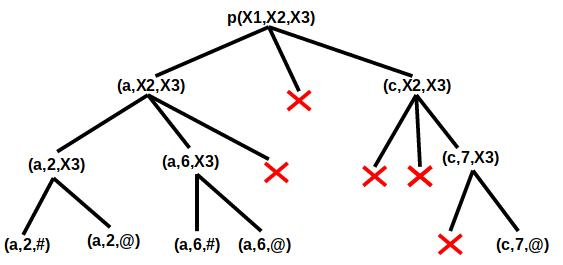
\includegraphics[width=0.950\textwidth, height=0.8\textheight]{figures/ilustra_backtracking_03.jpg}
%\caption{Realizar buscas com regiões reduzidas -- promissoras (regiões factíveis de soluções)}
\end{center}
\end{figure}
\textcolor{red}{Exercício: descubra os domínios possíveis de \texttt{X1}, \texttt{X2} e \texttt{X3}}
\end{frame}

s
\begin{frame}[fragile]
\frametitle{Ilustrando o \textit{Backtracking} -- 03}

\begin{figure}[!htb]
\begin{center}
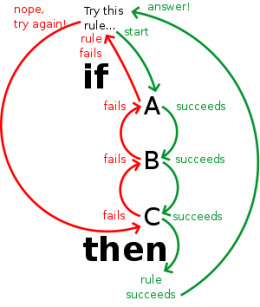
\includegraphics[width=0.60\textwidth, height=0.75\textheight]{figures/ilustra_backtracking_02.jpg}
%\caption{Realizar buscas com regiões reduzidas -- promissoras (regiões factíveis de soluções)}
\end{center}
\end{figure}

\end{frame}





%%%%%%%%%%%%%%%%%%%%%%%%%%%%%%%%%%%%%%%%%%%%%%%%%%%%%%%%%%%%%%%%%%%%%%%%%%%%%%%%%%%%%%%%%%

\begin{frame}[fragile]

\frametitle{Exemplos}
    
Tomando como exemplo uma relação de parentesco, como a seguinte:
% usar antecendente,sucessor, descendente etc.
        \begin{lstlisting}[frame=single]
index(-,-) (+,-) (-,+)
antecedente(ana,maria).
antecedente(pedro,maria).
antecedente(maria,paula).
antecedente(paula,lucas).
antecedente(lucas, eduarda).

index(-)
mulher(ana).
mulher(maria).
mulher(paula).
mulher(eduarda).
homem(pedro).
homem(lucas).

mae(X,Y) ?=> antecedente(X,Y), mulher(X).
pai(X,Y) ?=> antecedente(X,Y), homem(X).
avos(X,Y) ?=> antecedente(X,Z), antecedente(Z,Y).
sucessor(X,Y) ?=> antecedente(Y,X).
sucessor(X,Y) ?=> antecedente(Y,Z), sucessor(X,Z).
        \end{lstlisting}
    
\end{frame}


%%%%%%%%%%%%%%%%%%%%%%%%%%%%%%%%%%%%%%%%%%%%%%%%%%%%%%%%%%%%%%%%%%%%%%%%%%%%%%%%%%%%%%%%%%


\begin{frame}[fragile]
\frametitle{Exercícios}
    
    \begin{itemize}
        \item Uma chamada do tipo $mae(maria, X)$, seria como perguntar ao compilador
        "Maria é mãe de quem ?".
        
        \item Nesse caso o compilador iria testar cada possível valor que pudesse ser 
        unificado com $X$ que pudesse satisfazer a regra $mae(maria,X)$.
        
        \item Ou seja, seria como se estivéssemos perguntando:
        
        \begin{itemize}
            \item "Maria é mãe de Ana ?".
            
            \item "Maria é mãe de Paula ?".
            
            \item "Maria é mãe de Pedro ?".
            
    
        \end{itemize}
        
    \end{itemize}
    
\end{frame}




\begin{frame}[fragile]
\frametitle{Reflexões}


\begin{itemize}
\item A recursão é o paradigma das linguagens declarativas como Haskell, Prolog, Picat, ... etc
 
 \pause
 \item As regras recursivas são construídas com uma ou mais \textit{regras aterradas}, que \textbf{sempre vem antes} das demais
 regras recursivas, as  quais podem ou não terem o \textit{backtracking} habilitados (\textbf{\texttt{?=>}})
 
 
 \pause
 \item A avaliação destas regras \textbf{são sempre da esquerda para direita}, ocorrendo o \textit{backtracking} em caso de falha ou de uma nova resposta
  
  \pause
 \item As regras recursivas com \textit{backtracking} habilitados ( \textbf{\texttt{?=>}} ), apenas
 para regras predicativas. As funções não admitem \textit{backtracking}!
 
  \pause
 \item A metodologia destas regras e sua construção, seguem  esquemas mais
 avançados da programação declarativa
 
   \pause
 \item O \textbf{\textit{main}} é uma regra predicativa que pode conter ou não argumentos.
 
 
\end{itemize}

\end{frame}
%%%%%%%%%%%%%%%%%%%%%%%%%%%%%%%%%%%%%%%%%%%%%%%%%%%%%%%%%%%%%%%%%%%%%%%%%%%%%%%%%%%%%%%%%%
